\section{Introduction}

Most previous work on hierarchical RL considers either the finite-horizon setting or the infinite-horizon setting with discounted rewards.
The average-reward setting is better suited for cyclical tasks characterized by continuous experience.
In the few works on hierarchical RL in the average-reward setting, either the low-level tasks are assumed to be solved beforehand~\citep{Fruit2017,Fruit2017b,Wan2021a} or they % low-level tasks 
have important restrictions that severely reduce their applicability, e.g.~a single initial state~\citep{Ghavamzadeh2007}. It is therefore an open question how to develop algorithms for hierarchical RL in the average-reward setting
%with the average-reward criterion
in order to learn the low-level and high-level tasks simultaneously.


In this chapter we describe a novel framework for hierarchical RL in the average-reward setting that simultaneously solves low-level and high-level tasks. Concretely, considering the class of Linearly-solvable Markov Decision Processes (LMDPs)~\citep{Todorov2006}. The method here developed is an extension of the episodic case, described in the previous chapter, to the average-reward setting. Even though the compositionality property for LMDPs or methods of similar flavor have been proposed in RL~\cite{Hunt2019,Niekerk2019,NangueTasse2020} and in combination with hierarchical RL in the finite-horizon setting~\cite{Jonsson2016,Saxe2017,Infante2022}, adapting this idea to the average-reward setting requires careful analysis and poses a new challenge.


%% VICEN
% LMDPs are a class of restricted MDPs for which the Bellman equation can be exactly transformed into a linear equation. This class of problems plays a key role in the framework of RL as probabilistic inference~\cite{Kappen2012,Levine2018}.
% One of the properties of LMDPs is compositionality: one can compute the solution to a novel task from the solutions to previously solved tasks without learning~\citep{Todorov2009a}. 
%In addition to many other properties, for LMDPs it is possible to compose a solution to a novel task from the solutions to previously solved task without learning~\citep{Todorov2009a}.


%%% PREVIOUS
% Since the Bellman optimality equations are linear for LMDPs, it is possible to compose a solution to a novel task from the solutions to previously solved task without learning~\citep{Todorov2009a}. Compositionality has been previously exploited for hierarchical reinforcement learning for LMDPs in the finite-horizon setting~\citep{Infante2022}, but adapting the idea to the average-reward setting requires careful analysis.

Similarly to the first-exit case and unlike most frameworks for hierarchical RL, this approach does not decompose the policy, only the value function. Hence the agent never chooses a subtask to solve, and instead uses the subtasks to compose the value function of the high-level task. 
This avoids introducing non-stationarity at the higher level when updating the low-level policies.

\section{Contributions}
In this chapter we make the following contributions:
\begin{itemize}
  \item To develop a hierarchical framework that learns the low-level and  the high-level tasks simultaneously in the average-reward setting, without imposing additional restrictions on the low-level tasks.
    \item To propose two novel algorithms for solving hierarchical RL in the average reward setting: the first one is based on the eigenvector approach used for solving LMDPs. The second is an online variant in which an agent learns simultaneously the low-level and high-level tasks.
%  \item Representing low-level tasks as finite-horizon rather than average-reward decision processes.
    \item To provide two main theoretical contributions FOR LMDPs: convergence proofs for both differential soft TD-learning for (non-hierarchical) LMDPs and also for the eigenvector approach in the hierarchical case.
%  \item Proving the convergence of average-reward RL in non-hierarchical LMDPs.
  %\item Applying compositionality for reinforcement learning in the average-reward setting.
\end{itemize}

This work is the first that extends the combination of compositionality and hierarchical RL to the average-reward setting.

\section{Related work}
Most research on hierarchical RL formulates problems as a Semi-Markov Decision Process (SMDP) with options~\citep{Sutton1999} or the MAXQ decomposition~\citep{Dietterich2000}.

\citet{Fruit2017} and~\cite{Fruit2017b} propose algorithms for solving SMDPs with options in the average-reward setting, proving that the regret of their algorithms is polynomial in the size of the SMDP components, which may be smaller than the components of the underlying Markov Decision Process (MDP).
\citet{Wan2021a} present a version of differential Q-learning for SMDPs with options in the average-reward setting, proving that differential Q-learning converges to the optimal policy.
However, the above works assumes that the option policies are given prior to learning.
\citet{Ghavamzadeh2007} propose a framework for hierarchical average-reward RL based on the MAXQ decomposition, in which low-level tasks are also modeled as average-reward decision processes.
However, since the distribution over initial states can change as the high-level policy changes, the authors restrict low-level tasks to have a single initial state.

In the previous chapter combine the compositionality of LMDPs with the equivalence of low-level tasks to develop a framework for hierarchical RL in the finite-horizon setting.

In contrast, our hierarchical framework based on LMDPs can represent the globally optimal policy.

\section{Alternative method for solving an ALMDP}

An alternative method for solving an ALMDP $\cL$ is to transform it to a first-exit LMDP. 
Given a reference state $s^*$ and an original ALMDP $\cL=\langle\cS,\kernel,\cR\rangle$, define a first-exit LMDP $\cL'=\langle\cS\setminus\{s^*\},\{s^*\}, \kernel',\cR',\cJ'\rangle$, where $\kernel'(s'|s)=\kernel(s'|s)$ for all state pairs $(s,s')\in(\cS\setminus\{s^*\})\times\cS$, and $\cJ(s^*)=0$ (implying $z(s^*)=1$). By inspection of~\eqref{eq:boe_z_lmdp} and~\eqref{eq:boe_z_almdp}, we observe that the Bellman optimality equation of $\cL'$ is identical to that of $\cL$ if $\cR'(s)=\cR(s)-\rho$. Even though the agent has no prior knowledge of the exponentiated gain $\Gamma = e^{\eta\rho}$, we perform binary search to find $\Gamma$. For a given estimate $\widehat\Gamma$ of $\Gamma$, after solving $\cL'$, $\widehat \Gamma z(s^*)$ is compared to $e^{\eta\cR(s^*)}\sum_s\kernel(s|s^*)z(s)$. If $\widehat \Gamma z(s^*)$ is greater, then $\widehat\Gamma$ is too large, else it is too small.

Alternatively, when $\kernel$ and $\cR$ are not known, an estimate $\widehat v$ of the optimal value $v$ and an estimate $\widehat\rho$ of the optimal gain $\rho$ are kept using \textit{differential soft TD-learning}, similar to differential Q-learning~\citep{Wan2021}. We collect $(s_t, r_t, s_{t+1})$ generated by the estimated policy $\widehat\pi$ derived from $\widehat v$ as in \eqref{eq:lmdp_optimal_policy}. The update rules for $\widehat v$ and $\widehat \rho$ from \eqref{eq:boe_almdp} are as follows
\begin{align}
    \widehat{v}_{t+1}(s_t) &\gets \widehat{v}_t(s_t) + \alpha_t \delta_t,
    \label{eq:halmdps_main_v_td_update}\\
    \widehat{\rho}_{t+1} &\gets \widehat{\rho}_t + \lambda \alpha_t \delta_t.\label{eq:halmdps_main_rho_td_update}
    \end{align}
Here, the TD error $\delta_t$ is given by
\begin{align*}
\delta_t &= r_t - \widehat{\rho}_t - \frac 1 \eta \log \frac {\widehat{\pi}_t(s_{t+1}|s_t)} {\kernel(s_{t+1}|s_t)} + \widehat{v}_t(s_{t+1}) - \widehat{v}_t(s_t)\\
 &= r_t - \widehat{\rho}_t + \frac 1 \eta \log \sum_{s'\in\cS} \kernel(s'|s_t) e^{\eta \widehat{v}_t(s')} - \widehat{v}_t(s_t).
\end{align*}
% The learning rates $\alpha_t$ and $\beta_t$ can be chosen independently.
Note that both updates use the same TD error. At any time, we can retrieve the estimates of $\widehat z$ and $\widehat\Gamma$ by exponentiating $\widehat v$ and $\widehat \rho$, respectively.


\begin{theorem}
    Under mild assumptions, differential soft TD-learning in~\eqref{eq:halmdps_main_v_td_update} and~\eqref{eq:halmdps_main_rho_td_update} converges to the optimal values of $v$ and $\rho$ in $\cL$. \label{theo:almdps}
\end{theorem}

\begin{proof}[Proof sketch]
The proof is adapted from the proof of convergence of differential Q-learning~\cite{Abounadi2001,Wan2021}, which requires the ALMDP to be communicating (Assumption~\ref{ass:communicating}).
Define a Bellman operator $T$ as
\[
T(v)(s) = \cR(s) + \frac 1 \eta \log \sum_{s'\in\cS} \kernel(s'|s) e^{ \eta v(s') }.
\]
To adapt the previous proof, it is sufficient to show that $T$ is a non-expansion in the max norm, i.e.~$\infnorm{T(x)-T(y)} \leq \infnorm{x - y}$ for each $x, y\in\real^{|\cS|}$, and that $T$ satisfies $T(x + c\mathds{1}) = T(x) + c\mathds{1}$ for each $x\in\real^{|\cS|}$ and constant $c\in\real$, where $\mathds{1}$ is $|\cS|$-dimensional vector of all ones.
For completeness, the full proof appears in Appendix~\ref{proof:theo_almdps}.
\end{proof}


\begin{figure*}
  \begin{center}
  \begin{adjustbox}{width=0.4\textwidth}
    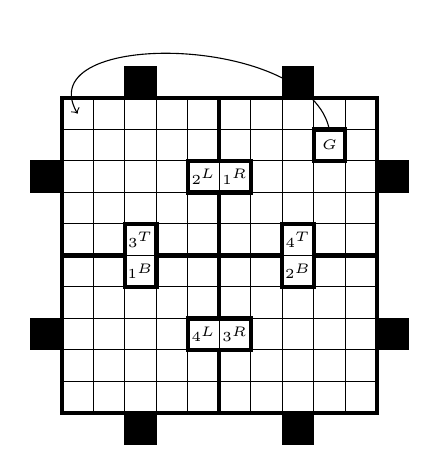
\begin{tikzpicture}
      \draw[step=0.4,thin,shift={(0.2,0.2)}] (0.8,0.8) grid (4.8,4.8);
      \draw[ultra thick] (1,1) rectangle (5,5);
      \draw[ultra thick] (3,1) -- (3,1.8);
      \draw[ultra thick] (3,2.2) -- (3,3.8);
      \draw[ultra thick] (3,4.2) -- (3,5);
      \draw[ultra thick] (1,3) -- (1.8,3);
      \draw[ultra thick] (2.2,3) -- (3.8,3);
      \draw[ultra thick] (4.2,3) -- (5,3);

      \draw[fill] (0.6,1.8) rectangle (1,2.2);
      \draw[fill] (0.6,3.8) rectangle (1,4.2);
      \draw[fill] (1.8,5) rectangle (2.2,5.4);
      \draw[fill] (1.8,0.6) rectangle (2.2,1);
      \draw[fill] (3.8,0.6) rectangle (4.2,1);
      \draw[fill] (5,1.8) rectangle (5.4,2.2);
      \draw[fill] (5,3.8) rectangle (5.4,4.2);
      \draw[fill] (3.8,5) rectangle (4.2,5.4);

      \draw[ultra thick] (4.2,4.2) rectangle (4.6,4.6);
      \draw[ultra thick] (3.8,2.6) rectangle (4.2,3.4);
      \draw[ultra thick] (1.8,2.6) rectangle (2.2,3.4);
      \draw[ultra thick] (2.6,3.8) rectangle (3.4,4.2);
      \draw[ultra thick] (2.6,1.8) rectangle (3.4,2.2);

      \node (R) at (1.2,4.8) {} ;
      \node (G) at (4.4,4.4) {\tiny $G$};
      \node at (2,3.2) {\tiny $3^T$};
      \node at (2,2.8) {\tiny $1^B$};
      \node at (4,3.2) {\tiny $4^T$};
      \node at (4,2.8) {\tiny $2^B$};
      \node at (2.8,4) {\tiny $2^L$};
      \node at (2.8,2) {\tiny $4^L$};
      \node at (3.2,4) {\tiny $1^R$};
      \node at (3.2,2) {\tiny $3^R$};

    %   \draw[step=0.4,thin,shift={(0.2,0)}] (8.799,1.999) grid (10.8,4);
    %   \draw[ultra thick] (9,3.2) -- (8.6,3.2) -- (8.6,2.8) -- (9,2.8) -- (9,2) -- (9.8,2);
    %   \draw[ultra thick] (9,3.2) -- (9,4) -- (9.8,4) -- (9.8,4.4) -- (10.2,4.4) -- (10.2,4);
    %   \draw[ultra thick] (10.2,4) -- (11,4) -- (11,3.2) -- (11.4,3.2) -- (11.4,2.8) -- (11,2.8);
    %   \draw[ultra thick] (9.8,2) -- (9.8,1.6) -- (10.2,1.6) -- (10.2,2) -- (11,2) -- (11,2.8);
    %   \draw[ultra thick] (10.2,3.2) rectangle (10.6,3.6);

    %   \node at (10.4,3.4) {\small $G$};
    %   \node at (8.8,3)    {\small $L$};
    %   \node at (11.2,3)   {\small $R$};
    %   \node at (10,1.8)   {\small $B$};
    %   \node at (10,4.2)   {\small $T$};

    %   \node at (3,0.7) {\Large a)};
    %   \node at (10,0.7) {\Large b)};

      \draw [->] (G.north) to [out=100,in=120] (R.center);
    \end{tikzpicture}
  \end{adjustbox}
  \end{center}
  \caption{An example $4$-room ALMDP that shows the adaptation of the previously introduced N-room domain to the average-reward setting. \\}
  \label{fig:halmdps_example}
\end{figure*}

\section{Hierarchical Average-Reward LMDPs}

In this section we present our approach for hierarchical average-reward LMDPs. The idea is to take advantage of the similarity of the value functions in the first-exit and average-reward settings, and use compositionality to compose the value functions of the subtask LMDPs without additional learning.

%\subsubsection{Hierarchical Decomposition}
\subsection{Hierarchical Decomposition}
Consider an ALMDP $\langle\cS,\kernel,\cR\rangle$. Similarly to the previous chapter, we assume the state space $\cS$ is partitioned into subsets $\left\{\cS_i\right\}^L_{i=1}$, with each partition $\cS_i$ inducing
a first-exit LMDP $\cL_i = \langle\cS_i, \cT_i, \kernel_i, \cR_i,\cJ_i\rangle$.
The components of each such subtask $\cL_i$ are defined as follows:
\begin{itemize}
  \item The set of states is $\cS_i$.
  \item The set of terminal states $\cT_i=\{\tau\in\cS\setminus\cS_i: \exists s\in\cS_i, \kernel(\tau|s)>0\}$ contains states not in $\cS_i$ that are reachable in one step from any state inside the partition.
  \item The transition function $\kernel_i$ and reward function $\cR_i$ are projections of $\kernel$ and $\cR-\widehat\rho$ onto $\cS_i$, where $\widehat\rho$ is a gain estimate.
  \item $\cJ_i$ is defined for each $\tau\in\cT_i$ as $\cJ_i(\tau)=\widehat v(\tau)$, where $\widehat v$ is a current value estimate (hence $z_i(\tau)=e^{\eta\widehat v(\tau)} = \widehat z(\tau)$ is defined by a current exponentiated value estimate $\widehat z$).
\end{itemize}
The Bellman optimality equations of each subtask $\cL_i$ are given by
\begin{equation}\label{eq:halmdps_subtask}
  z_i(s) = e^{\eta \cR_i(s)} \sum_{s'} \kernel_i(s'|s) z_i(s') \;\; \forall s\in\cS_i.
\end{equation}
By inspection of the Bellman optimality equations in~\eqref{eq:boe_z_almdp} and~\eqref{eq:halmdps_subtask}, they are equal if $\cR_i(s)=\cR(s)-\rho$. Thus, if $z_i(\tau)=z(\tau)$ for each $\tau\in\cT_i$ then the solution of the subtask $\cL_i$ corresponds to the optimal solution for each $s\in\cS_i$. However, in general neither $\rho$ nor $z(\tau)$ are known prior to learning and, therefore, estimates $\widehat\rho$ and $\widehat z(\tau)$ must be used instead. Each subtask $\cL_i$ can be seen as being {\it parameterized\/} on the value estimates $\widehat z(\tau)$ for each $\tau\in\cT_j$ and the gain estimate $\widehat\rho$. Every time that $\widehat z(\tau)$, $\tau\in\cT_i$, and $\widehat\rho$ change, we can obtain a new value estimate for each $s\in\cS_i$ by solving the subtask for the new parameters.

%\subsection{Subtask compositionality}
\subsection{Subtask Compositionality}
In the same way as in the first-exit case, it is impractical to solve each subtask $\cL_i$ every time the estimate $\widehat z(\tau)$ changes for $\tau\in\cT_j$. In order to alleviate this, we leverage compositionality for LMDPs. Again, the key insight is to build a basis of value functions that can be combined to obtain the solution for the subtasks.

Consider a subtask $\cL_i=\langle\cS_i,\cT_i,\kernel_i,\cR_i,\cJ_i\rangle$ and let $n=|\cT_i|$.  Let $\{\cL_i^1,\ldots,\cL_i^n\}$ be $n$ base LMDPs that are first-exit LMDPs and terminate in $\cT_i$. These base LMDPs only differ from $\cL_i$ in the reward of each terminal state $\tau^k\in\cT_i$. For all $s\in\cS_i$, the reward for each $\cL_i^k$ is by definition $\cR_i(s)=\cR(s)-\widehat\rho$ for all $s\in\cS_i$, while at terminal states $\tau\in\cT_i$ let the reward function is $z_i^k(\tau;\widehat\rho)=1$ if $\tau=\tau^k$ and $z_i^k(\tau;\widehat\rho)=0$ otherwise. Thus, the base LMDPs are parameterized by the gain estimate $\widehat\rho$. This is equivalent to setting the reward to $\cJ_i^k(\tau)=0$ if $\tau=\tau_k$ and $\cJ_i^k(\tau)=-\infty$ otherwise. Intuitively, each base LMDP solves the subtask of reaching one specific terminal state $\tau_k\in\cT_i$.

Assume that the solution $z_i^1(\cdot;\rho),\ldots,z_i^n(\cdot;\rho)$ for the base-LMDPs (for the optimal gain $\rho$) is available as well as the optimal value $z(\tau^k)$ of the original ALMDP for each terminal state $\tau^k\in\cT_i$. Then by compositionality we could represent the value function of each terminal state can be represented as a weighted combination of the subtasks:
\begin{equation}
  z(\tau) = \sum_{k=1}^n w_k z_i^k(\tau;\rho) =  \sum_{k=1}^n z(\tau^k) z_i^k(\tau;\rho) \;\;\forall\tau\in\cT_i.
  \label{eq:comp_terminal}
\end{equation}

Clearly, the RHS in the previous expression evaluates to $z(\tau)$ since $z(\tau^k) z_i^k(\tau;\rho) = z(\tau)\cdot 1$ when $\tau = \tau^k$, and
$z(\tau^k) z_i^k(\tau;\rho) = z(\tau^k)\cdot 0$ otherwise.

Thanks to compositionality, it is also possible to represent the value function for each subtask state $s\in\cS_i$ as
\begin{equation}
  z(s) = \sum_{k=1}^n z(\tau^k) z_i^k(s;\rho)\;\;\forall s\in\cS_i.
  \label{eq:halmdps_comp_internal}
\end{equation}
It is significant to remark that the base LMDPs depend on the gain $\rho$ by the definition of the reward function. This parameter is not known prior to learning. The subtasks in practice are solved for the latest estimate $\widehat\rho$ and must be re-learned for every update of this parameter until convergence.
\subsection{Efficiency of the value representation}
 Similar to previous work~\citep{Wen2020,Infante2022} the equivalence of subtasks is exploited to learn more efficiently. Let $\cC=\{\cC_1,\ldots,\cC_C\}$, $C\leq L$, be a set of equivalence classes, i.e.~a partition of the set of subtasks $\{\cL_1,\ldots,\cL_L\}$ such that all subtasks in a given partition are equivalent.
As before, a set of exit states as $\cE=\cup_{i=1}^L\cT_i$ is also defined.
Due to the decomposition, there is no need to keep an explicit value estimate $\widehat z(s)$ for every state $s\in\cS$. Instead, it is sufficient to keep a value function for exit states $\widehat z_\cE: \cE\rightarrow\real$ and a value function for each base LMDP of each equivalence class. This is enough to represent the value for any state $s\in\cS$ using the compositionality expression in~\eqref{eq:halmdps_comp_internal}.

Again, let $K=\max_{i=1} ^L\lvert\cS_i\rvert$,  $N=\max_{i=1} ^L\lvert\cT_i\rvert$ and $E=\lvert\cE\rvert$. Then only $O(KN)$ values are needed to represent the base LMDPs of a subtask, and the value function can be represented with $O(CKN + E)$ values. The decomposition leads to an efficient representation of the value function whenever $CKN + E \ll \lvert\cS\rvert$. This is achieved when there are few equivalence classes, the size of each subtask is small (in terms of the number of states) and there are relatively few exit states.

  % {\bf Example}: Consider the $4$-room example depicted in Figure~\ref{fig:halmdps_example}. Here there is a single equivalence class that generalizes all the rooms. Therefore, a single subclass is represented with $5\times 5$ states. This subtask induces $5$ base-LMDPs with terminal states in $G,L,R,T,B$. Besides, there is a total of 

  %{\bf Example 1:} 
  \paragraph{Example 1}: Figure~\ref{fig:halmdps_example} shows an 4-room LMDP adapted to the average-reward seeing. When reaching the state marked $G$, separate from the room but reachable in one step from the highlighted location, the agent receives a reward of $0$ and, in contrast to the first-exit case, the system transitions to a restart state (top left corner). In all other states the reward is $-1$. To behave optimally, thus, the agent should visit the state marked as $G$ as often as possible. The other aspects of the decomposition, remain equal to the first-exit setting. % as those of the subtasks.
  %Hence the number of equivalent subtasks is $C=1$, the number of non-terminal and terminal states of subtasks is $K=25$ and $N=5$, respectively, and the number of exit states is $E=9$.
    %In the 4-room example, t
    % There are five base LMDPs with value functions $z^G$, $z^L$, $z^R$, $z^T$ and $z^B$, respectively. Given an initial value estimate $\widehat{z}_\cE$ for each exit state in $\cE$, a value estimate of any state in the top left room is given by $\widehat{z}(s)=\widehat{z}_\cE(1^B) z^B(s) + \widehat{z}_\cE(1^R) z^R(s)$, where $\widehat{z}_\cE(G)=\widehat{z}_\cE(L)=\widehat{z}_\cE(T)=0$ is used to indicate that the terminal states $G$, $L$ and $T$ are not reachable in the top left room. 
    In this case, the total number of values needed to store the optimal value function is $E+CKN=9+125=134$, and the base LMDPs are faster to learn since they have smaller state space.
    %We need $CKN = 125$ values to store the value functions of the 5 base LMDPs, and $E=9$ values to store the value estimates of all exit states. Although this is more than the 100 states of the original LMDP, if we increase the number of rooms to $X\times Y$, the term $CKN$ is a constant as long as all rooms have equivalent dynamics, and the number of exit states is $E=(2X-1)(2Y-1)$, which is much smaller than the $25XY$ total states. For $10\times 10$ rooms, the value function decomposition requires $486$ values to represent the values of $2{,}500$ states.


\section{Algorithms}
In this section we describe two novel algorithms for solving hierarchical ALMDPs. The first is a two-stage eigenvector approach that relies on first solving the subtasks. The second is an online algorithm in which an agent simultaneously learns the subtasks, the gain and the exit values from samples $(s_t, r_t, s_{t+1})$.
Once again it is important to remark that the values for states $s\notin\cE$ are not explicitly represented.

\subsection{Eigenvector approach}

In the episodic case, the base LMDPs are only solved once, and the solutions are then reused to compute the value function $z_\cE$ on exit states (see section~\ref{section:hlmdps_eigenvector_episodic}). However, in the case of ALMDPs, the reward functions of base LMDPs depend on the current gain estimate $\widehat\rho$, which is initially unknown. 

% I think the duration part is false!!!

%If we could estimate the expected {\em duration} $d_i(s)$ of each subtask $\cL_i$ from each state $s\in\cS_i$, we could use the duration to adjust the value estimate $\widehat z(s)$ of $s$ according to the current gain estimate $\widehat\Gamma$ by a factor $\widehat \Gamma^{d_i(s)}$. The duration can be recursively defined as $d_i(\tau)=0$ for each $\tau\in\cT_i$ and
%\[
%d_i(s) = 1 + \sum_{s'} \pi_i(s'|s) d_i(s').
%\]
%However, even though the subtask policy $\pi_i$ can be expressed in terms of the base LMDP policies $\pi_i^k$, we have been unable to formulate $d_i$ as a composition of the durations $d_i^k$ of base LMDPs, and hence the duration would have to be recomputed each time we resolve a subtask $\cL_i$, which is inefficient.

%We describe in Algorithm~\ref{alg:halmdps_eigenvector}. 
The eigenvector approach for solving hierarchical ALMDPs appears in Algorithm~\ref{alg:halmdps_eigenvector}. The intuition is that in each iteration, we first solve the subtasks for the latest estimate of the exponentiated gain $\widehat\Gamma$. For this, the base LMDPs are solved with~\eqref{eq:halmdps_subtask} using with the current value of $\widehat\rho$. Then~\eqref{eq:halmdps_comp_internal} is applied, restricted to $\cE$ to obtain an estimate of the value for the exit states. This yields the system of linear equations
\begin{equation}
    {\bf z_\cE} = G_\cE {\bf z_\cE}.\label{eq:halmdps_eigenvector}
\end{equation}
Here, the matrix $G_\cE\in\real^{\lvert\cE\rvert\times \lvert\cE\rvert}$ contains the optimal values of the base LMDPs and has elements defined as in~\eqref{eq:halmdps_comp_internal}. The previously introduced idea to transform the ALMDP $\cL$ to a first-exit LMDP $\cL'$ parameterized on the estimated gain $\widehat\rho$ is used, and the optimal exponentiated gain $\Gamma$ is found using binary search. There is a reference state $s^*\in\cS$ (which is by definition an exit state) and on which binary search is performed to find $\Gamma$.

\begin{algorithm}[!b]
  \caption{Eigenvector approach to solving a hierarchical ALMDP.}
  \setstretch{1.2}
  \begin{algorithmic}[1]
    %\Require{An ALMDP $\cL=\langle\cS,\cP,\cR\rangle$, a partition $\cS_1,\ldots,\cS_L$ of $\cS$, inducing a set of exit states $\cE$, reference state $s^\star$.}

    %\Procedure{\textsc{SolveALMDP}}{$\cL,\cS_1,\ldots,\cS_L,\cE,\epsilon,\eta$}
    \State{{\bf Input:} $\cL,\cS_1,\ldots,\cS_L,\cE,\epsilon,\eta$}
    \State $\text{lo}\gets 0$, $\text{hi}\gets 1$
    \While {$\text{hi} - \text{lo} > \epsilon$}
    \State $\widehat\Gamma \gets (\text{hi} + \text{lo}) \mathbin{/} 2$
    %\For{each subtask $\cL_i$}
    %\State Form the matrix $G_i = G_j(\eta,\widehat{\Gamma}_k)$
    %\State Solve the Bellman optimality equation $\widehat{\bf z}_i = G_i\widehat{\bf z}_i^+$
    %\EndFor
    \State Solve base LMDPs $\cL_j^1,\ldots,\cL_j^n$ for each equivalence class $\cC_j$
    \State Form the matrix $G_\cE$ from the optimal value functions
    \State Solve the system of equations  ${\bf \widehat z_\cE} = G_\cE {\bf\widehat z_\cE}$
    \If {$ \widehat\Gamma \widehat z_\cE(s^*) > e^{\eta \cR(s^*)} \sum_{s\in\cS} \kernel(s\lvert s^*) \widehat z_\cE(s)$}
    \State $\text{hi}\gets \widehat\Gamma$
    \Else \State $\text{lo}\gets \widehat\Gamma$
    \EndIf
    \vspace*{3pt}
    \EndWhile
    \State \Return value functions of all base LMDPs, ${\bf \widehat z_\cE}$
    %\EndProcedure
  \end{algorithmic}
  \label{alg:halmdps_eigenvector}
\end{algorithm}

\begin{theorem}\label{thm:converge}
    Algorithm~\ref{alg:halmdps_eigenvector} converges to the optimal value function $z$ of $\cL$ as $\epsilon\to 0$.
\end{theorem}
% The proof of Theorem~\ref{thm:converge} appears in Appendix~\ref{proof:theo_h}.

First note that the optimal value function $z$ of $\cL$ exists and is unique due to Assumption~\ref{ass:communicating}. Due to the equivalence between $\cL$ and the corresponding first-exit LMDP $\cL'$, this implies that $\cL'$ has a unique solution $z(\cdot;\rho)$ when the estimated gain $\widehat\rho$ equals $\rho$, and that this solution equals $z(\cdot;\rho)=z$, the optimal solution to $\cL$.

\begin{lemma}\label{lemma:monotonicity}
     Given a first-exit LMDP $\cL'$ parameterized on $\widehat\rho$, the optimal value $z(s;\widehat\rho)$ of each non-terminal state $s\in\cS$ is strictly monotonically decreasing in $\widehat\rho$.
\end{lemma}

\begin{proof}
Strict monotonicity requires that there exists $\varepsilon>0$ such that $\linebreak{z(s;\widehat\rho - \varepsilon) > z(s;\widehat\rho) > z(s;\widehat\rho+\varepsilon)}$ when $\varepsilon\rightarrow 0$. The first inequality is proven by induction; the second is analogous. The base case is given by the terminal states $\tau\in\cT$, for which $z(\tau;\widehat\rho - \varepsilon) = z(\tau;\widehat\rho)$. The inductive case is given by
\begin{align*}
    z(s;\widehat\rho-\varepsilon) &= e^{\eta(\cR(s) - (\widehat\rho -\varepsilon))}\sum_{s'\in\cS}\kernel(s'\lvert s) z(s';\widehat\rho- \varepsilon)\\
      &\geq e^{\eta\varepsilon} e^{\eta(\cR(s) - \rho))}\sum_{s'\in\cS}\kernel(s'\lvert s) z(s';\widehat\rho)\\
      &= e^{\eta\varepsilon} z(s;\widehat\rho) > z(s;\widehat\rho).
\end{align*}
This concludes the proof.
\end{proof}

As a consequence of Lemma~\ref{lemma:monotonicity}, $\cL'$ has a unique solution $z(\cdot,\widehat\rho)$ for each $\widehat\rho\geq\rho$, since the values $z(\cdot,\widehat\rho)$ decrease as $\widehat\rho$ increases. In contrast, there may be values of $\widehat\rho>\rho$ for which power iteration does not converge.

\begin{restatable}{lemma}{optimality}
Given a subtask $\cL_i$, if the optimal value of each terminal state $\tau\in\cT_i$ equals its optimal value in $\cL$, i.e. $z_i(\tau) = z(\tau)$, and the optimal gain $\rho$ in $\cL$ is known, then the optimal value of each non-terminal state $s\in\cS_i$ is unique and equals $z_i(s)=z(s)$.
    \label{lemma:optimality}
\end{restatable}

\begin{proof} Since $\cR_i$ and $\kernel_i$ are restrictions of $\cR-\rho$ and $\kernel$, respectively, to $\cS_i$, then
\begin{align*}
    z_i(s) &= e^{\eta\cR_i(s)}\sum_{s'}\kernel_i(s'\lvert s) z_i(s') = e^{\eta(\cR(s) - \rho)}\sum_{s'}\kernel(s'\lvert s) z_i(s'), \nonumber
\end{align*}
which is the same Bellman equation as for $z(s)$. Assuming that $z_i(\tau) = z(\tau)$ for each $\tau\in\cT$, directly yields that $z_i(s)=z(s)$ for each non-terminal state $s\in\cS_i$.
\end{proof}

\begin{corollary}\label{cor:uniqueness}
    If the optimal gain $\rho$ in $\cL$ is known, each base LMDP $\cL_j^k$ has a unique solution $z_j^k(\cdot;\rho)$.
\end{corollary}

\begin{proof} From \eqref{eq:halmdps_comp_internal}, the optimal values of subtask states satisfy
\[
  z(s) = \sum_{k=1}^n z(\tau^k) z_i^k(s;\rho)\;\;\forall s\in\cS_i.
\]
Due to Lemma~\ref{lemma:optimality}, the optimal value $z(s)$ is unique, which is only possible if $z_i^k(s;\rho)$ is unique for each $\tau^k\in\cT_i$.
\end{proof}

Combined with Lemma~\ref{lemma:monotonicity}, Corollary \ref{cor:uniqueness} implies that each base LMDP $\cL_j^k$ has a unique solution $z_j^k(\cdot;\widehat\rho)$ whenever $\widehat\rho\geq\rho$.

\begin{lemma}
For $\widehat\rho\geq\rho$, the equation ${\bf \widehat z_\cE} = G_\cE {\bf\widehat z_\cE}$ has a unique solution that equals $z_\cE(\tau)=z(\tau;\widehat\rho)$ for each exit $\tau\in\cE$, where $z(\cdot;\widehat\rho)$ is the unique value of the first-exit LMDP $\cL'$ for $\widehat\rho$.
\end{lemma}

\begin{proof}
At convergence, due to \eqref{eq:halmdps_comp_internal} it has to hold for each non-terminal exit $\tau\in\cE$ that
\[
  z_\cE(\tau) = \sum_{k=1}^n z_\cE(\tau^k) z_i^k(s;\widehat\rho)\;\;\forall s\in\cS_i,
\]
where each $\tau^k$ is also an exit and $z_i^k(s;\widehat\rho)$ is well-defined and unique since $\widehat\rho\geq\rho$. This equation is satisfied when $z_\cE(\tau)=z(\tau;\widehat\rho)$ for each exit. Since $z(\cdot;\widehat\rho)$ is unique, this is the only solution.
\end{proof}

Now we have all the ingredients to prove Theorem~\ref{thm:converge}. When $\widehat\rho\geq\rho$ (or equivalently, $\widehat\Gamma\geq\Gamma$), each base LMDP has a unique solution, and $z_\cE$ is also unique. Moreover, when $\widehat\rho>\rho$, the condition on line 8 is true, which causes binary search to discard all values greater than $\widehat\rho$. If the base LMDPs or $z_\cE$ do not have a unique solution, it means that $\widehat\rho$ is too small, and hence all values less than $\widehat\rho$ can be discarded. Since the solution $z(\cdot;\widehat\rho)$ is monotonically decreasing in $\widehat\rho$, binary search is guaranteed to find the optimal gain $\rho$ within a factor of $\epsilon$.

\subsection{Online hierarchical algorithm}
 In the online case (see Algorithm~\ref{alg:halmdps_online}), we keep an estimate of the exponentiated gain $\widehat\Gamma=e^{\eta\widehat\rho}$ which is updated every timestep. We also keep estimates of the value functions of the base LMDPs $\widehat z_i^1(\cdot;\widehat\rho),\ldots,\widehat z_i^n(\cdot;\widehat\rho)$ for each equivalence class $\cC_i$, and estimates of the value function on exit states $\widehat z_\cE$.  All the base LMDPs of the same equivalence class can be updated with the same sample using intra-task learning with the appropriate {\it importance sampling weights\/}~\citep{Jonsson2016}. We only update the estimates of the exit states upon visitation. In that case, the compositionality expression in~\eqref{eq:halmdps_comp_internal} is used to derive the following update:
\begin{equation}
  \widehat z_\cE(s)\gets (1-\alpha_\ell) \widehat z_\cE(s) + \alpha_\ell \sum_{k=1}^n \widehat z_\cE(\tau^k) \widehat z_i^k(s;\rho).
  \label{eq:halmdps_update_exit}
\end{equation}
Here, $\alpha_\ell$ is the learning rate. Each of the learned components (i.e., gain, base LMDPs and exit state value estimates) maintain independent learning rates.

\begin{algorithm}[!htpb]
  \caption{Online hierarchical algorithm.}
  \setstretch{1.12}
  \begin{algorithmic}[1]
    \State{{\bf Input:} $\cL,\cS_1,\ldots,\cS_L,\cE,s_0,\epsilon,\eta$}
    \State $t \gets 0$, $\widehat{\Gamma} \gets 1$
    \While {{\it not terminate}}
    \State Observe $(s_{t}, r_{t}, s_{t+1})\sim\widehat\pi_t$
    \State Update $\widehat z_j^1(\cdot;\widehat\rho),\ldots,\widehat z_j^n(\cdot;\widehat\rho)$ using Equation~\eqref{eq:halmdps_main_v_td_update}
    \State Compute $\widehat z(s_t)$ and $\sum_{s'}\kernel(s'|s_t)\widehat z(s')$ using Equation \eqref{eq:halmdps_comp_internal}
    \State Update $\widehat\Gamma$ using Equation~\eqref{eq:halmdps_main_rho_td_update}
    \If{$s_t\in\cE$}
    \State Update $\widehat z_\cE(s_t)$ using Equation~\eqref{eq:halmdps_update_exit}
    \EndIf
    \EndWhile
    \State \Return value functions of all base LMDPs, ${\widehat z_\cE}$

  \end{algorithmic}
  \label{alg:halmdps_online}
\end{algorithm}

\section{Experiments}

We now present the experimental results for the two benchmark control problems introduced in the previous chapter and explain how we adapt them to the continuing case. \footnote{Code available at \url{https://github.com/guillermoim/halmdps}}.
% Vicenc: We report some results for Algorithm~\ref{alg:halmdps_eigenvector}. These are  simple experiments meant to show that the hierarchical eigenvector method indeed converges to the optimal (exponentiated) gain up to an arbitrary precision, and, consequently, to the optimal value function.

Then, we compare Algorithm~\ref{alg:halmdps_online} against differential soft TD-learning in the flat representation of the ALMDP. Similarly to the first-exit case, the metric used for the experiments Mean Absolute Error (MAE) between the estimated value function $\widehat z$ and the true optimal value function $z$, taken exclusively at the exit states. For each algorithm, the results are averaged over five seeds. Along with the average, the standard deviation is also reported. Here, the learning rates decay every $n$ samples, and are given by the expression $\alpha_\ell \leftarrow k \alpha_\ell$, where $k$ is the decay factor. The hyperparameters $n$ and $k$ are optimized per instance. \todo{Why no $V_2$ and $V_3$.}

Note that, while the updates rules for differential Z-learning (Equations~\eqref{eq:diff_update_z} and~\eqref{eq:diff_update_gamma}) are in the exponential domain, the here derived soft TD-learning updates (Equations~\eqref{eq:halmdps_main_v_td_update} and~\eqref{eq:halmdps_main_rho_td_update}) are in the logarithmic domain. This has some advantages such as using a single TD-error for both the value function and the gain update. Similarly, for our hierarchical approach we can keep an estimate of the value function $\widehat v_{\cE}$ in the logarithmic domain. In such a case, the update rule~\eqref{eq:halmdps_update_exit} can be expressed as 
\begin{equation*}
    \widehat v_{\cE}(s)\gets (1-\alpha_\ell) \widehat v_\cE(s) + \alpha_\ell\frac{1}{\eta} \log\Big(\sum_{k=1}^n e^{\eta \widehat  v_\cE(\tau^k)} \widehat z_i^k(s;\rho)\Big).
\end{equation*}
Simultaneously, the gain estimate is updated with~\eqref{eq:halmdps_main_rho_td_update}. Recall that, at any moment, these estimates can be expressed in the exponential domain with $\widehat z_\cE(s)=e^{\eta\widehat v_\cE(s)}$ and $\widehat\Gamma=e^{\eta\widehat\rho}$. Our experimental results show that this version of the hierarchical algorithm is more stable.

\begin{figure}[!ht]
  \centering
  \includegraphics*[width=0.49\textwidth]{figures/chapter2/eigenvectors/lmdp-nroom-3.pdf}
  \includegraphics*[width=0.49\textwidth]{figures/chapter2/eigenvectors/lmdp-taxi-8.pdf}
  \caption{Error in $\widehat\Gamma$ per iteration for Algorithm~\ref{alg:halmdps_eigenvector}.}
  \label{fig:halmdps_eigenvectos}
 \end{figure}

Besides the learning error for the higher level, the learning error for the subtasks and the gain are also disclosed for the logarithmic and exponential domains. These results should be able to partly show better stability in the logarithmic domain. In contrast to the first-exit case, now there is a three-way dependency during learning between the (optimal) gain, value function of the subtasks and values of the exit states which makes hierarchical learning in the average-reward setting more challenging.  

  \subsection{N-room domain}
 As in the episodic case, there are some `goal' states with high reward (i.e. $0$). When the agent enters a goal state, the next action causes it to receive the given reward and transition to a {\it restart\/} location. The number of rooms as well as the size of the rooms are varied to obtain different instances of the problem.   
 
 Figure~\ref{fig:halmdps_eigenvectos} (left) shows the results for a single run of Algorithm~\ref{alg:halmdps_eigenvector} in the largest instance of this domain. We report the absolute error of the estimate $\widehat\Gamma$ at each iteration. We observe that the binary search procedure finds the optimal value up to an arbitrary precision which can be then used to compute the optimal value function. 
 
 The results for learning are in Figure~\ref{fig:halmdps_nrooms}. The difference in the error scale in the figures is due to the initialization of the base LMDPs. We observe that both the hierarchical approaches (logarithmic and exponential domains) outperfom the flat learner by several orders of magnitude (note the logarithmic scale).  The average reward setting poses an extra challenge since the `sparsity' of the reward can make the estimates of the gain oscillate. This ultimately has an impact on the estimates of the base LMDPs and the value estimates of the exit states, and it is likely the reason why in Figure~\ref{fig:halmdps_taxi} the error increases before decreasing down to zero. Nonetheless, the logarithmic version of the algorithm converges faster. This is likely to be caused by a faster convergence of $\widehat \Gamma$. The bottom row of Figure~\ref{fig:halmdps_nrooms} shows that the magnitude of this error behaves more stably in the logarithmic version, which might cause of the error in the subtasks (middle row of Figure~\ref{fig:halmdps_nrooms}) to be better upperbounded. Consequently, this might translate in a better convergence in the high-level (top row of Figure~\ref{fig:halmdps_nrooms}).

  \begin{sidewaysfigure}
  \centering
  \includegraphics*[width=0.32\textwidth]{figures/chapter2/online/nrooms_3_3_1.png}
  \includegraphics*[width=0.32\textwidth]{figures/chapter2/online/nrooms_5_5_1.png}
  \includegraphics*[width=0.32\textwidth]{figures/chapter2/online/nrooms_8_8_1.png}

  \includegraphics*[width=0.32\textwidth]{figures/chapter2/online/nrooms_3_3_subtasks_1.png}
  \includegraphics*[width=0.32\textwidth]{figures/chapter2/online/nrooms_5_5_subtasks_1.png}
  \includegraphics*[width=0.32\textwidth]{figures/chapter2/online/nrooms_8_8_subtasks_1.png}

  \includegraphics*[width=0.32\textwidth]{figures/chapter2/online/nrooms_3_3_gammas_1.png}
  \includegraphics*[width=0.32\textwidth]{figures/chapter2/online/nrooms_5_5_gammas_1.png}
  \includegraphics*[width=0.32\textwidth]{figures/chapter2/online/nrooms_8_8_gammas_1.png}


  \caption{Results in N-room when varying the number of rooms and the size of the rooms.}
  \label{fig:halmdps_nrooms}
  \end{sidewaysfigure}
  


  \subsection{Taxi domain}
  Adapting this environment to the continuing case is more natural. In this variant of the original domain~\citep{Dietterich2000}, once the passenger has been dropped off, the system transitions to a state in which the driver is in the last drop-off location, but a new passenger appears randomly at another location. Hence the driver immediately receives a new assignment after having successfully completed the previous one. 

  The results of the eigenvector algortihm in Figure~\ref{fig:halmdps_eigenvectos} (right) shows the same pattern as in the N-room domain. In this domain, the results for the learning algirthm Figure~\ref{fig:halmdps_taxi} also provide the same conclusions as in the N-room domain: the hierarhical approaches need less number of samples to converge, and the logarithmic version seems to be faster and more stable.



  \begin{figure}[!hb]
    \begin{center}
        \includegraphics*[width=0.49\textwidth]{figures/chapter2/online/taxi_5_1.png}
        \includegraphics*[width=0.49\textwidth]{figures/chapter2/online/taxi_8_1.png}
        \includegraphics*[width=0.49\textwidth]{figures/chapter2/online/taxi_5_subtask_1.png}
        \includegraphics*[width=0.49\textwidth]{figures/chapter2/online/taxi_8_subtask_1.png}
        \includegraphics*[width=0.49\textwidth]{figures/chapter2/online/taxi_5_gammas_1.png}
        \includegraphics*[width=0.49\textwidth]{figures/chapter2/online/taxi_8_gammas_1.png}
        % \includegraphics*[width=0.49\textwidth]{figures/chapter2/online/taxi_8_subtasks_1.pdf}
        \caption{Results for $5 \times 5$ (top) and $8 \times 8$ (bottom) grids of the Taxi domain.}
          \label{fig:halmdps_taxi}
    \end{center}
  \end{figure}
  %In this case, the adaptation to an infinite-horizon task is more natural. Once the passenger has been dropped off, the system transitions to a state in which the driver is in the last dropoff location, but a new passenger appears at another location. %Hence the driver immediately receives a new assignment after having successfully completed the previous one.

% \begin{figure*}[!bt]
%   \centering
%   \includegraphics*[width=0.32\textwidth]{pictures/nrooms_3_3-1.png}
%   \includegraphics*[width=0.32\textwidth]{pictures/nrooms_5_5-1.png}
%   \includegraphics*[width=0.32\textwidth]{pictures/nrooms_8_8-1.png}
%   \caption{ Results in N-room when varying the number of rooms and the size of the rooms.}
%   \label{fig:nrooms}
% \end{figure*}

% \begin{figure}[!htp]
%   \centering
%   \includegraphics*[width=0.33\textwidth]{pictures/taxi_5-1.png}
%   \includegraphics*[width=0.33\textwidth]{pictures/taxi_10-1.png}
%   \caption{Results for $5 \times 5$ (left) and $10 \times 10$ (right) grids of the Taxi domain.}
%   \label{fig:taxi}

% \end{figure}


\section{Conclusion}

In this chapter we present a novel framework for hierarchical average-reward reinforcement learning which makes it possible to learn the low-level and high-level tasks simultaneously. 
We propose an eigenvector approach and an online algorithm for solving problems in our hierarchical framework, and show that the former converges to the optimal value function. We provide experimental results of the hierarchical updates both in the logarithmic and exponential domains that show that the logarithmic domain behaves more stably. The experimental results also show that either of the hierarchical versions outperforms a flat learner by several orders of magnitude.
As a by-product of our analysis, we also provide a convergence theorem in the non-hierarchical case for average-reward LMDPs, which to the extent of our knowledge, was not previously done. In the future we would like to prove convergence also for the proposed online algorithm.
